%
% Available class options:
%	- printformat: to produce the final document to be printed. Omit to produce electronic document.
%	- checkreferences: set to check for unused citations
%	- grayfigures: use gray figures
%	- I would prefer to set openright
%
\documentclass[11pt,openany,twoside,printformat]{book}
%
% load preamble-min, and apply geometry
% ----------------------------------------------------------------------
% Check options
% ----------------------------------------------------------------------
\makeatletter%
\newif\ifprintformat
\@ifclasswith{book}{printformat}{\printformattrue}{\printformatfalse}
\newif\ifcheckreferences
\@ifclasswith{book}{checkreferences}{\checkreferencestrue}{\checkreferencesfalse}
\newif\ifgrayfigures
\@ifclasswith{book}{grayfigures}{\grayfigurestrue}{\grayfiguresfalse}
\makeatother
\ifgrayfigures
\def\figpref{gray-}
\else
\def\figpref{}
\fi
% Line spacing
% ----------------------------------------------------------------------
\usepackage{setspace}
\renewcommand{\baselinestretch}{1.0}% default line spacing, up to 1.2 looks nice
%
% Geometry def
% ----------------------------------------------------------------------
% good ref: http://practicaltypography.com
%			and: http://mirrors.ctan.org/macros/latex/contrib/geometry/geometry.pdf
%
\ifdefined\thegeometrytextwidth
\else
	\def\thegeometrytextwidth{6.0in}
\fi
\ifdefined\thegeometryinit
\else
	\def\thegeometryinit{paper=a4paper,headheight=16pt,marginparwidth=60pt,textwidth=\thegeometrytextwidth,textheight=8.5in,heightrounded,vmarginratio=8:10}
\fi
%
\ifdefined\thegeometryextra
\else
	%\ifprintformat
		%\def\thegeometryextra{hmarginratio=3:4,bindingoffset=0.5cm}% margins for printing
	%\else
		\def\thegeometryextra{hcentering,bindingoffset=0cm}% margins for electronic document
	%\fi
\fi
%
\def\thegeometry{\thegeometryinit,\thegeometryextra}
%
% BLANK PAGE
% ----------------------------------------------------------------------
\newcounter{totalblankpages}
\setcounter{totalblankpages}{0}% set it to something just in case
\newcounter{mypagecount}% create a new counter
\setcounter{mypagecount}{0}% set it to something just in case
\newenvironment{interlude}{% create a new environment for the unnumbered section(s)
\clearpage
\setcounter{mypagecount}{\value{page}}% use the new counter we created to hold the page count at the start of the unnumbered section
\thispagestyle{empty}% we want this page to be empty (adjust to use a modified page style)
\pagestyle{empty}% use the same style for subsequent pages in the unnumbered section
}{%
\clearpage
\setcounter{page}{\value{mypagecount}}% restore the incremented value to the official tally of pages so the page numbering continues correctly
}
\ifprintformat
	\newcommand\blankpage{%
	\begin{interlude}
	\null
	\stepcounter{totalblankpages}
	\end{interlude}
	}
\else
	\newcommand\blankpage{%
	%
	}
\fi

\usepackage[\thegeometry]{geometry}
\usepackage{layout}% to get and/or display page layout details
%
% Fonts
% ----------------------------------------------------------------------
\usepackage{iftex}
\ifPDFTeX
	\usepackage{cmap}% make pdf files searchable and copyable
	\usepackage[utf8]{inputenc}
	\usepackage[T1]{fontenc}
	\usepackage{lmodern}
	\usepackage{amsmath,amsfonts,amssymb}
	%
	\usepackage{isomath}% english standards
	%
	\def\myfancyfont{}
\else
	\usepackage{amsmath,amssymb}
	\usepackage[no-math]{fontspec}
	%
	\defaultfontfeatures{Ligatures=TeX}
	%
	% If latin modern fonts are not found using XeTex in linux:
	%	- [ubuntu]Make sure lmodern package is installed
	%	- [ubuntu] create a new file 09-texmffonts.conf in /etc/fonts/conf.avail/ and sym link it to ../conf.d
	%	- [ubuntu] put in that file the directories /usr/share/texmf/fonts/opentype|truetype|type1 and /usr/share/texlive/texmf-dist/fonts/opentype|truetype|type1
	%	- [arch] Install the aur package otf-latin-modern
	%	- [arch] This should be optional and the config should already be there, otherwise put directories might be instead /usr/share/texmf-dist/fonts/opentype|truetype|type1 and /usr/local/share/texmf/fonts/opentype|truetype|type1
	%	- [arch] Make sure the sym link to the tex font config exists in /etc/fonts/conf.d
	%	- If you have added a font conf then run fc-cache -f -v
	\setmainfont[
		Numbers=Proportional,
		Ligatures={TeX},
		SlantedFont={Latin Modern Roman Slanted},
		SmallCapsFont={Latin Modern Roman Caps},
		ItalicFeatures={SmallCapsFeatures={FakeSlant=0.2}}
	]{Latin Modern Roman}
	\setsansfont[
		Scale=MatchLowercase
	]{Latin Modern Sans}% Note that there is no latin modern Sans Caps font nor slanted one.
	\setmonofont[
		Scale=MatchLowercase
	]{Latin Modern Mono Light}
	%
	%\usepackage[math-style=ISO,bold-style=ISO]{unicode-math}% english standards 
	\usepackage[math-style=french]{unicode-math}% french standards 
	\setmathfont[Path=./fonts/math/]{latinmodern-math.otf}
	%
	\ifLuaTeX
	\else
	\fi
	%
	\newfontfamily\myfancyfont[
		ItalicFont=EBGaramond12-Italic.otf,
		Ligatures={Rare, Historic, TeX},
		Contextuals=Alternate,
		RawFeature={+dlig},
		ItalicFeatures={Style=Swash}
	]{EBGaramond12-Regular.otf}
\fi

% Some maths defs
% ----------------------------------------------------------------------
\newcommand*\diff{\mathop{}\!\mathrm{d}}
\newcommand*\Diff[1]{\mathop{}\!\mathrm{d^#1}}

% Miscellaneous - 1
% ----------------------------------------------------------------------
%\usepackage{flafter}% forces floats to appear only after the place where they are defined
\usepackage{verbatim}% for block comment
\usepackage{graphicx}
\graphicspath{{./figures/}}
\usepackage{booktabs,tabularx}% better column width for tabular environment
\usepackage{multirow}% multirow env for tabular
\usepackage{xcolor}
%\usepackage{tikz}% used in cover page
%\usetikzlibrary{calc}% needed for coordinate calculation in tikz
\usepackage{tcolorbox}% used in cover page
\tcbuselibrary{skins}% lib for tcolorbox
\usepackage{shadowtext}% used in cover page
%\usepackage{listings}% code source formatting
\usepackage{algorithm}% float wrapper
\usepackage{algorithmicx}% typesetting environment
\usepackage[noend]{algpseudocode}% layout for algorithmicx
\usepackage{cite}
\usepackage{IEEEtrantools}% needed to use \bstctlcite with IEEEtran
\ifcheckreferences
	\usepackage[ignoreunlbld]{refcheck}% checks for unused citations and more 
\fi
\usepackage[bottom]{footmisc}% make sure foot notes have constant distance with fancy foot when using raggedbottom 
\usepackage{fancyhdr}% fancy headers and footers
%\usepackage{shorttoc}% short table of contents
%\usepackage[tiny, md, sc]{titlesec}
\usepackage{titlesec}
\pagestyle{plain}
\usepackage{titling}% title, author, date and thanks commands
\usepackage[Conny]{fncychap}% nice chap titles: Lenny, Conny, Bjornstrup
%\usepackage[palatino]{quotchap}
\usepackage{lettrine}% lettrine command
\usepackage[titletoc]{appendix}
\usepackage[tight,nice]{units}% provides commands: \unit, \unitfrac and \nicefrac
\usepackage[titles]{tocloft}% table of content format
\setlength{\cftbeforesecskip}{5pt}
%\renewcommand{\cftchapafterpnum}{\vspace{5pt}}
\renewcommand{\cftsecleader}{\cftdotfill{\cftdotsep}}
\renewcommand{\cftchapfont}{\normalsize \scshape}
\renewcommand{\cftchappagefont}{\normalsize \scshape}
%
\begingroup\expandafter\expandafter\expandafter\endgroup
\expandafter\ifx\csname IncludeInRelease\endcsname\relax
  \usepackage{fixltx2e}% include this only for releases prior to 2015
\fi
%
\usepackage{ragged2e}
%
\parindent 15pt
%
\widowpenalty=9000
\clubpenalty=9000
%\brokenpenalty=501
\raggedbottom% make all pages the height of the text on that page. No need for extra vertical space (especially between section title and text).
%
%\renewcommand{\thefootnote}{\fnsymbol{footnote}}
%
\hyphenation{net-works}% correct bad hyphenation here
%
\setcounter{secnumdepth}{3}% 1 = sections only, 2 = sections + subsections, 3 = sections + subsections + subsubsections
\setcounter{tocdepth}{2}
%
% hyperref related packages
% ----------------------------------------------------------------------
% note: You might need to add hyperindex=false if "see" and "seealso" commands are not working in index generation.
% However you should not need this, as it should have been fixed in ./preamble/index.xdy
% See: https://en.wikibooks.org/wiki/Talk:LaTeX/Indexing#Texindy.2C_hyperref_and_textbf.2C_textit_modifiers
% and see: http://geekographie.maieul.net/190
%\usepackage[hidelinks,hyperindex=false]{hyperref}
\usepackage[hidelinks]{hyperref}
\usepackage{bookmark}
%
% Acronyms
% ----------------------------------------------------------------------
\usepackage[xindy={language=french, codepage=utf8}, style=altlist, nonumberlist]{glossaries}% glossaries
\usepackage{glossary-mcols}
\renewcommand*{\acronymtype}{acronym}
\newglossary[alg]{acronym}{acr}{acn}{\acronymname}
\makeglossaries
%
% locale related packages
% ----------------------------------------------------------------------
\usepackage[labelfont={footnotesize,up,bf,sf,singlespacing},
			textfont={footnotesize,up,md,sf,singlespacing},
			justification={justified},
			singlelinecheck=false,
			margin=0pt,
			figurewithin=chapter,
			tablewithin=chapter]{caption}% caption package which sets figure, table caption font, format, name etc.
%
\usepackage{polyglossia}
\setmainlanguage{french}
\setotherlanguage{english}
% We need arabic locale for abstract-ar, however we do not load it using polyglossia. It loads bidi package which breaks fncychap and maybe other packages.
%
% Miscellaneous - 2
% ----------------------------------------------------------------------
% 
% Definitions Commands
% ----------------------------------------------------------------------
\makeatletter
\ifdefined\theauthor
	\def\@author{\theauthor}
\else
	\def\author#1{\gdef\@author{#1}}
	\def\theauthor{\@author}
\fi
\def\titlefrench#1{\gdef\@titlefrench{#1}}
\def\thetitlefrench{\@titlefrench}
\def\titleenglish#1{\gdef\@titleenglish{#1}}
\def\thetitleenglish{\@titleenglish}
\def\keywordsfrench#1{\gdef\@keywordsfrench{#1}}
\def\thekeywordsfrench{\@keywordsfrench}
\def\keywordsenglish#1{\gdef\@keywordsenglish{#1}}
\def\thekeywordsenglish{\@keywordsenglish}
\def\advisor#1{\gdef\@advisor{#1}}
\def\theadvisor{\@advisor}
\def\degreeyear#1{\gdef\@degreeyear{#1}}
\def\thedegreeyear{\@degreeyear}
\def\degreemonth#1{\gdef\@degreemonth{#1}}
\def\thedegreemonth{\@degreemonth}
\def\degreeday#1{\gdef\@degreeday{#1}}
\def\thedegreeday{\@degreeday}
\makeatother


%
% Styling Commands
% ----------------------------------------------------------------------
%

\definecolor{chaptergrey}{rgb}{0.1000, 0.1600, 0.0060}%
\definecolor{hdrrule}{rgb}{0.4000, 0.4000, 0.4000}%

\fancypagestyle{empty}{
	\fancyhf{}
	\cfoot{}%\thepage}
	\renewcommand{\headrulewidth}{0pt}% header horizontal line
}

\fancypagestyle{emptynonum}{
	\fancyhf{}
	\cfoot{}
	\renewcommand{\headrulewidth}{0pt}% header horizontal line
}

\makeatletter
\@ifclasswith{book}{openany}{%
	\renewcommand*{\cleardoublepage}{\clearpage}%
}{%
	\renewcommand*{\cleardoublepage}{
		\clearpage
		\if@twoside
			\ifodd
				\c@page
			\else
				\hbox{}%
				\thispagestyle{empty}%
				
				\newpage%
				\if@twocolumn\hbox{}
					\newpage
				\fi
			\fi
		\fi
	}%
}
\makeatother

% page header
% ----------------------------------------------------------------------
\fancyhf{}% clear header
%\fancyhead[RO,LE]{\thepage}
%\fancyhead[LO]{\normalfont\nouppercase{\rightmark}}
%\fancyhead[RE]{\normalfont\nouppercase{\leftmark}}

\newcounter{realpagenum}
\fancyhead[RO,RE]{%
\setcounter{realpagenum}{\value{page}}%
\addtocounter{realpagenum}{\value{totalblankpages}}%
\ifodd\value{realpagenum}{\thepage}\else{\normalfont\nouppercase{\leftmark}}\fi%
}
\fancyhead[LO,LE]{%
\setcounter{realpagenum}{\value{page}}%
\addtocounter{realpagenum}{\value{totalblankpages}}%
\ifodd\value{realpagenum}{\normalfont\nouppercase{\rightmark}}\else{\thepage}\fi%
}

\pretocmd{\headrule}{\color{hdrrule}}{}{}
%\renewcommand{\headrulewidth}{0pt}% no horizontal line in headers
%\renewcommand{\footrulewidth}{0.4pt}% footer horizontal line
\pagestyle{fancy}
%
%\def\markchapter#1{\markboth{\MakeUppercase{#1}}{\MakeUppercase{#1}}}
\def\markchapter#1{\markboth{#1}{#1}}
\def\addchapter#1{\cleardoublepage\phantomsection{}\markchapter{#1}}% adds chapter but does not list it in toc
\def\addchaptertoc#1{\addchapter{#1}\addcontentsline{toc}{chapter}{#1}}% adds chapter and lists it in toc
\pretocmd{\tableofcontents}{\addchaptertoc{\contentsname}}{}{}
\newcommand{\listspart}{\addcontentsline{toc}{chapter}{Listes}}
\newif\ifListsStarted
\ListsStartedfalse
\newcommand{\listsname}{Listes}
\newcommand{\checkListsStarted}{\ifListsStarted\else\addcontentsline{toc}{chapter}{\listsname}\ListsStartedtrue\fi}
\pretocmd{\listoffigures}{\addchapter{\listfigurename}\checkListsStarted\addcontentsline{toc}{section}{\listfigurename}}{}{}
\pretocmd{\listoftables}{\addchapter{\listtablename}\checkListsStarted\addcontentsline{toc}{section}{\listtablename}}{}{}
\pretocmd{\printnomenclature}{\addchapter{\nomname}\checkListsStarted\addcontentsline{toc}{section}{\nomname}}{}{}
\newcommand\listacronymname{Liste des abréviations, sigles et acronymes}
\newcommand\listofacronyms{\addchapter{\listacronymname}\checkListsStarted\addcontentsline{toc}{section}{\listacronymname}\printglossary[type=\acronymtype,title=\listacronymname,style=mcoltree,nogroupskip]}
\pretocmd{\printindex}{\addchaptertoc{\indexname}}{}{}
\pretocmd{\bibliography}{\addchaptertoc{\bibname}}{}{}
\makeatletter
\newcounter{ChapterCounter}
\renewcommand{\theHsection}{\theChapterCounter.\the\value{section}}% used by hyperref, we modified this to make sure we provide unique string when using chapter*
\newif\ifChapterIsStarred
\renewcommand{\thesection}{\ifChapterIsStarred\else\the\value{chapter}.\fi\the\value{section}}% we modified this to hide chapter number when using chapter*
\def\startschapternotext#1{%
	\ChapterIsStarredtrue%
	\stepcounter{ChapterCounter}%
	\phantomsection\markchapter{#1}%
	\setcounter{section}{0}%
}
\pretocmd{\@schapter}{%
	\startschapternotext{#1}
}{}{}
\pretocmd{\@chapter}{%
	\ChapterIsStarredfalse%
	\stepcounter{ChapterCounter}%
}{}{}
\if@twoside
	% chapter title in even pages and section in odd pages
	\renewcommand{\chaptermark}[1]{\markboth{\chaptername\ \thechapter.\ #1}{\chaptername\ \thechapter.\ #1}}
	\renewcommand{\sectionmark}[1]{\markright{\thesection\ #1}}
\else
	% chapter title in both odd and even pages and no section
	\renewcommand{\chaptermark}[1]{\markboth{\chaptername\ \thechapter.\ #1}{\chaptername\ \thechapter.\ #1}}
	\renewcommand{\sectionmark}[1]{}
\fi
\makeatother

% front style
% ----------------------------------------------------------------------
\renewcommand{\frontmatter}{
	\pagenumbering{roman}
}

% main style
% ----------------------------------------------------------------------
\renewcommand{\mainmatter}{
	\cleardoublepage
	\setcounter{page}{1}
	\pagenumbering{arabic}
}

% back style
% ----------------------------------------------------------------------
\renewcommand{\backmatter}{
	\cleardoublepage
}

% etc
% ----------------------------------------------------------------------

\newcommand{\nullpart}{
	\bookmarksetup{startatroot}% Use bookmark package so that all following chapters appear in the root (no part)
}

\newenvironment{copyrightpage}{
	\clearpage{}% appears at the verso of the title page with year, author, the publisher, the ISSN number, etc. 
	\null\vspace*{\fill}
	\begin{center}
}{
	\end{center}
	\null
}

\newenvironment{dedications}{
	\cleardoublepage
	\null\vspace*{\stretch{1}}
	\begin{flushright}
	\large\itshape\myfancyfont
}{
	\end{flushright}
	\vspace*{\stretch{2}}\null
}

\newenvironment{abstract}{
	\par\noindent\textbf{\small\abstractname}%
	\par%
}{
}

\def\acknowledgmentsname{Remerciements}
\newenvironment{acknowledgments}{
	\chapter*{\acknowledgmentsname}
	\addcontentsline{toc}{chapter}{\acknowledgmentsname}
	\setstretch{1.2}
	\large\itshape
}{
}

\def\prefacename{Préface}
\newenvironment{preface}{
	\chapter*{\prefacename}
	\addcontentsline{toc}{chapter}{\prefacename}
}{
}

\def\listofpublicationsname{Nos publications}
\newenvironment{listofpublications}{
	\chapter*{\listofpublicationsname}
	\addcontentsline{toc}{chapter}{\listofpublicationsname}
}{
}

\newcommand{\inenglish}[1]{\textenglish{\textit{#1}}}% foreign langage for french should be in italic

\makeatletter
\def\setfigpath#1{\gdef\@figpath{#1}}
\def\figpath{\@figpath}
\makeatother

\captionsetup{%
	figurename=Figure,
	tablename=Tableau
}
%\AtBeginDocument{%
%\renewcommand\figurename{\textsc{Figure}}
%\renewcommand\tablename{\textsc{Tableau}}
%}

% Algorithms
% ----------------------------------------------------------------------
% numbering
\makeatletter 
\renewcommand\thealgorithm{\thechapter.\arabic{algorithm}} 
\@addtoreset{algorithm}{chapter} 
\makeatother

% locale
\makeatletter
\newcommand{\newalgname}[1]{%
  \renewcommand{\ALG@name}{#1}%
}
\newalgname{Algorithme}
\renewcommand{\listalgorithmname}{Liste des \ALG@name s}
\makeatother

\renewcommand{\algorithmicrequire}{\textbf{Entrée:}}
\renewcommand{\algorithmicensure}{\textbf{Sortie:}}
\renewcommand{\algorithmicend}{\textbf{fin}}
\renewcommand{\algorithmicif}{\textbf{si}}
\renewcommand{\algorithmicthen}{\textbf{alors}}
\renewcommand{\algorithmicelse}{\textbf{sinon}}
\renewcommand{\algorithmicfor}{\textbf{pour}}
\renewcommand{\algorithmicforall}{\textbf{pour chaque}}
\renewcommand{\algorithmicdo}{\textbf{faire}}
\renewcommand{\algorithmicwhile}{\textbf{tant que}}
\renewcommand{\algorithmicrepeat}{\textbf{répéter}}
\renewcommand{\algorithmicuntil}{\textbf{jusqu'à}}
\renewcommand{\algorithmicreturn}{\textbf{retourner}}
\newcommand{\algorithmicelsif}{\algorithmicelse\ \algorithmicif}
\newcommand{\algorithmicendif}{\algorithmicend\ \algorithmicif}
\newcommand{\algorithmicendfor}{\algorithmicend\ \algorithmicfor}


% other styling
% ----------------------------------------------------------------------

\newcommand{\enquote}[1]{«\,#1\,»}

\newcommand{\manualpagebreak}{\pagebreak}

% Copyright
% ----------------------------------------------------------------------
%\begin{copyrightpage}
%	\copyright{} \thedegreeyear{} \theauthor{}
%
%	TOUS DROITS RÉSERVÉS
%\end{copyrightpage}
% definitions
%
% Commands
% ----------------------------------------------------------------------
\makeatletter
\ifdefined\theauthor
	\def\@author{\theauthor}
\else
	\def\author#1{\gdef\@author{#1}}
	\def\theauthor{\@author}
\fi
\def\titlefrench#1{\gdef\@titlefrench{#1}}
\def\thetitlefrench{\@titlefrench}
\def\titleenglish#1{\gdef\@titleenglish{#1}}
\def\thetitleenglish{\@titleenglish}
\def\keywordsfrench#1{\gdef\@keywordsfrench{#1}}
\def\thekeywordsfrench{\@keywordsfrench}
\def\keywordsenglish#1{\gdef\@keywordsenglish{#1}}
\def\thekeywordsenglish{\@keywordsenglish}
\def\advisor#1{\gdef\@advisor{#1}}
\def\theadvisor{\@advisor}
\def\degreeyear#1{\gdef\@degreeyear{#1}}
\def\thedegreeyear{\@degreeyear}
\def\degreemonth#1{\gdef\@degreemonth{#1}}
\def\thedegreemonth{\@degreemonth}
\def\degreeday#1{\gdef\@degreeday{#1}}
\def\thedegreeday{\@degreeday}
\makeatother
%
% Values
% ----------------------------------------------------------------------
\date{\today}% define date as today
\titlefrench{Le titre du mémoire (modifiable dans preamble/definitions.tex)}
\keywordsfrench{Mot clé 1, Mot clé 2, Mot clé 3, Mot clé 4, Mot clé 5}
\titleenglish{The titre of the document in english}
\keywordsenglish{Keyword 1, Keyword 2, Keyword 3, Keyword 4, Keyword 5}
\author{Prénom NOM \textnormal{et} Prénom NOM}
\advisor{Prénom NOM}

% ... about the degree.
\degreeyear{2024}
\degreemonth{mai}
\degreeday{26}

% Acronyms
%

% Ajouter les acronymes utilisés dans le document ici
%
\newacronym{CPU}{CPU}{\inenglish{Central Processing Unit}}
\newacronym{TIC}{TIC}{Technologies de l'Information et des Communications}
\newacronym{VIM}{VIM}{\inenglish{Virtual Infrastructure Manager}}
\newacronym{VM}{VM}{Machine Virtuelle}

\glsaddall% add all glossary/acronym entries. Instead we could call the \gls{} command where appropriate.

% Set pdf meta data
\hypersetup{
	pdfencoding=auto,
    pdfauthor={\theauthor},
    pdftitle={\thetitlefrench},
    pdfkeywords={\thekeywordsfrench}
}





% It is recommended to either use XeTeX or LuaTeX
% We do not recommend using PDFTeX (and is now also not supported because of polyglossia usage)
%\RequireXeTeX{}

\usepackage{lipsum}
%\usepackage{mynotes}
%\usepackage{mwe}

\begin{document}
%
\frontmatter
% Page du titre
%
% Page du titre
%
\expandafter\newgeometry\expandafter{\thegeometryextra,headheight=0pt,marginparwidth=0pt,textwidth=7in,textheight=10in}
\begin{titlepage}\noindent{%
\thispagestyle{emptynonum}%
% logo
\begin{minipage}{0.2\textwidth}%
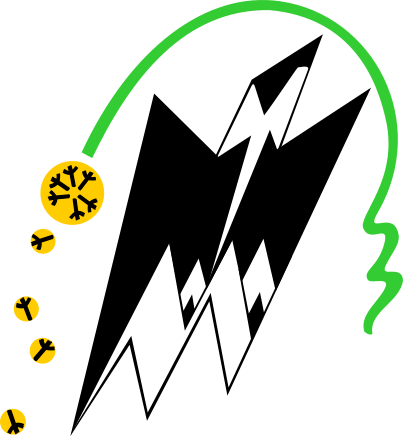
\includegraphics[width=1.1in]{univ-logo.png}
\end{minipage}% no new line
\begin{minipage}{0.8\textwidth}
\raggedleft
{
\bfseries
%\scriptsize
\footnotesize
\setstretch{1.0}
République Algérienne Démocratique et Populaire\\
Ministère de l'Enseignement Supérieur et de la Recherche Scientifique\\
Université Mouloud Mammeri de Tizi-Ouzou\\
Faculté de Génie Électrique et d'Informatique\\
Département d'Informatique\\
}
\end{minipage}%
% spacing
\par
\vspace*{1.0in}
%
\noindent{\begin{center}%
	\noindent{\shadowoffset{2pt}\shadowtext{\bfseries\Huge THÈSE}}\\
	\vspace*{10pt}
	\noindent{\large En vue de l'obtention du diplôme \\
	de Master 2 en Informatique}\\
	\vspace*{5pt}
	\noindent{\large\textnormal{Spécialité:} Systèmes Informatiques}\\
	\vspace*{25pt}
	\noindent{\large\textnormal{Présenté par:} {\bfseries\Large \theauthor}}\\
	\vspace*{5pt}
\end{center}}
% title
\noindent{\centering \begin{tcolorbox}[width=6in,
			text width=5.8in,
			halign=center,
			arc=3pt,
			outer arc=4pt
			boxrule=2pt,
			colback=black!3!white
		  ]%%
                  \bfseries\LARGE \thetitlefrench
\end{tcolorbox}}%
%
\vspace*{0pt}%
\noindent{\begin{center}\begin{minipage}{6.0in}\raggedleft\large{}\textnormal{Mémoire encadré par:} \theadvisor\end{minipage}\end{center}}
\par
%
\vspace*{30pt}
\noindent{\begin{center}\begin{minipage}{6.0in}\large{}Soutenu publiquement devant le jury composé de:\end{minipage}\end{center}}
\par
%
\begin{center}
	\setstretch{1.4}
	\large 
	\begin{tabularx}{6in}{l>{\arraybackslash\hspace{0.5in}}Xr}%{l>{\centering\arraybackslash}Xr}
		\hline
		Prénom NOM			& Pr. Univ. de Tizi-Ouzou	&	Président\\
		Prénom NOM			& MAA. Univ. de Tizi-Ouzou	&	Examinateur\\
		Prénom NOM			& MCA. Univ. de Tizi-Ouzou 	&	Examinateur\\
		\theadvisor			& MCB. Univ. de Tizi-Ouzou	&	Encadrant\\
		\hline
	\end{tabularx}
\end{center}
%
%
\vspace{30pt}
\begin{center}
\footnotesize
Copyright \copyright{} \thedegreeyear{} \theauthor{}.

TOUS DROITS RÉSERVÉS.
\end{center}
}\end{titlepage}

\restoregeometry
%
\blankpage
%\input{./frontmatter/copyright}%
% Preface
%
\begin{acknowledgments}

Lorem ipsum dolor sit amet, consectetur adipiscing elit. Phasellus suscipit nulla et mattis mattis. Curabitur vel tempor tellus. 
Fusce lacinia fringilla fringilla. Vestibulum in nulla at dolor malesuada viverra. 
Morbi fermentum justo neque, quis aliquam quam vehicula eu. Aenean eu pharetra risus. 
Cras id magna et mi malesuada porttitor. 

Aliquam varius, est et porttitor ultricies, massa mi rutrum velit, eu mattis felis leo in lorem.
Aenean feugiat commodo ex, vitae feugiat purus semper eget. Praesent at arcu viverra, suscipit metus quis, blandit eros.
Pellentesque a lacus sodales, lacinia ante at, condimentum eros. Nunc eu lacus tellus. In scelerisque eros ex,
quis suscipit augue pharetra porta. Nam aliquam congue metus nec bibendum. Quisque sed auctor nibh. 

Praesent consectetur est ut ultricies tempus. Integer placerat luctus lacinia.
Vestibulum ante ipsum primis in faucibus orci luctus et ultrices posuere cubilia curae;
Maecenas sapien nibh, egestas at eros vel, suscipit facilisis enim. Ut mollis eleifend ligula,
quis sagittis enim consequat nec. Phasellus non lectus a nulla gravida interdum sit amet non erat.
Nulla id luctus leo, sed consectetur magna. Cras tincidunt, lacus vel varius mollis, elit turpis finibus sem,
ac viverra dolor mi id leo. In tellus lorem, cursus in iaculis vel, tristique vitae lacus. Aenean at ornare felis.
Phasellus dapibus sit amet justo eu elementum. Orci varius natoque penatibus et magnis dis parturient montes,
nascetur ridiculus mus. Quisque iaculis mauris at lorem venenatis hendrerit. Vestibulum purus diam, sagittis sed mauris a,
congue efficitur lacus. Nullam suscipit justo et arcu porta lobortis. 

\vspace{10pt}

\begin{flushright}
En vous souhaitant une agréable lecture,

\theauthor{}.
\end{flushright}
\end{acknowledgments}
%
\blankpage
\cleardoublepage
\startschapternotext{Résumés}%
\addcontentsline{toc}{chapter}{Résumés}%
% Resumé en français
%
\begin{abstract}
\footnotesize

Lorem ipsum dolor sit amet, consectetur adipiscing elit. Phasellus suscipit nulla et mattis mattis. Curabitur vel tempor tellus. 
Fusce lacinia fringilla fringilla. Vestibulum in nulla at dolor malesuada viverra. 
Morbi fermentum justo neque, quis aliquam quam vehicula eu. Aenean eu pharetra risus. 
Cras id magna et mi malesuada porttitor. 

Aliquam varius, est et porttitor ultricies, massa mi rutrum velit, eu mattis felis leo in lorem.
Aenean feugiat commodo ex, vitae feugiat purus semper eget. Praesent at arcu viverra, suscipit metus quis, blandit eros.
Pellentesque a lacus sodales, lacinia ante at, condimentum eros. Nunc eu lacus tellus. In scelerisque eros ex,
quis suscipit augue pharetra porta. Nam aliquam congue metus nec bibendum. Quisque sed auctor nibh. 

\vspace{0pt}
{\textbf{{Mots clés:}} \thekeywordsfrench{}.}
\end{abstract}

\par\vspace{5pt}\par%
%\par\noindent\hfil\rule[0.5ex]{0.5\linewidth}{0.7pt}\hfil\par
% Abstract in English
%
\selectlanguage{english}
\begin{abstract}
\footnotesize

Lorem ipsum dolor sit amet, consectetur adipiscing elit. Phasellus suscipit nulla et mattis mattis. Curabitur vel tempor tellus. 
Fusce lacinia fringilla fringilla. Vestibulum in nulla at dolor malesuada viverra. 
Morbi fermentum justo neque, quis aliquam quam vehicula eu. Aenean eu pharetra risus. 
Cras id magna et mi malesuada porttitor. 

Aliquam varius, est et porttitor ultricies, massa mi rutrum velit, eu mattis felis leo in lorem.
Aenean feugiat commodo ex, vitae feugiat purus semper eget. Praesent at arcu viverra, suscipit metus quis, blandit eros.
Pellentesque a lacus sodales, lacinia ante at, condimentum eros. Nunc eu lacus tellus. In scelerisque eros ex,
quis suscipit augue pharetra porta. Nam aliquam congue metus nec bibendum. Quisque sed auctor nibh. 

\vspace{0pt}
{\textbf{{Keywords:}} \thekeywordsenglish{}.}
\end{abstract}
\selectlanguage{french}

\par\vspace{5pt}\par%
%\par\noindent\hfil\rule[0.5ex]{0.5\linewidth}{0.7pt}\hfil
%
\blankpage
% toc
% ----------------------------------------------------------------------
\renewcommand\contentsname{Table des matières}
\tableofcontents
\blankpage
% Chapters
% ----------------------------------------------------------------------
\mainmatter
% Introduction
%
\def\thischaptitle{Introduction générale}
\chapter*{\thischaptitle}
\addcontentsline{toc}{chapter}{\thischaptitle}
%
\section{Contexte}

Lorem ipsum dolor sit amet, consectetur adipiscing elit. Phasellus suscipit nulla et mattis mattis. Curabitur vel tempor tellus. 
Fusce lacinia fringilla fringilla. Vestibulum in nulla at dolor malesuada viverra. Morbi fermentum justo neque, quis aliquam quam vehicula eu. 
Aenean eu pharetra risus. Cras id magna et mi malesuada porttitor.

Aliquam varius, est et porttitor ultricies, massa mi rutrum velit, eu mattis felis leo in lorem. 
Aenean feugiat commodo ex, vitae feugiat purus semper eget. Praesent at arcu viverra, suscipit metus quis, blandit eros. 
Pellentesque a lacus sodales, lacinia ante at, condimentum eros. Nunc eu lacus tellus. In scelerisque eros ex, quis suscipit augue pharetra porta. 
Nam aliquam congue metus nec bibendum. Quisque sed auctor nibh.

Praesent consectetur est ut ultricies tempus. Integer placerat luctus lacinia. 
Vestibulum ante ipsum primis in faucibus orci luctus et ultrices posuere cubilia curae; Maecenas sapien nibh, egestas at eros vel, suscipit facilisis enim. 
Ut mollis eleifend ligula, quis sagittis enim consequat nec. Phasellus non lectus a nulla gravida interdum sit amet non erat. 
Nulla id luctus leo, sed consectetur magna. Cras tincidunt, lacus vel varius mollis, elit turpis finibus sem, ac viverra dolor mi id leo. 
In tellus lorem, cursus in iaculis vel, tristique vitae lacus. Aenean at ornare felis. Phasellus dapibus sit amet justo eu elementum. 
Orci varius natoque penatibus et magnis dis parturient montes, nascetur ridiculus mus. Quisque iaculis mauris at lorem venenatis hendrerit. 
Vestibulum purus diam, sagittis sed mauris a, congue efficitur lacus. Nullam suscipit justo et arcu porta lobortis.

In nec augue vel ligula sagittis pharetra et ac arcu. Vivamus rutrum, velit eget vulputate suscipit, augue tortor eleifend velit, a interdum metus lectus a mi. 
Aliquam erat volutpat. Sed euismod iaculis neque, bibendum tincidunt risus ultricies eget. 
In vel sem tincidunt dolor malesuada pellentesque eget a ligula. Curabitur tempus, leo a viverra euismod, ipsum velit viverra elit, in dictum sapien enim vitae nisi. Ut porttitor, lectus eu pellentesque aliquet, risus orci posuere justo, sit amet lobortis arcu justo at lacus. 
Nullam suscipit, ligula congue mollis suscipit, nisl massa imperdiet enim, eu porttitor libero felis sit amet sapien. 
Integer ac congue neque, id hendrerit sem. Morbi eleifend nibh feugiat ligula sagittis maximus.

Nulla sagittis sem et nisi rutrum, a ornare ligula placerat. Praesent scelerisque purus ac ex feugiat, auctor ultrices magna faucibus. 
Phasellus nec fermentum mi. Etiam vitae quam a leo malesuada facilisis. Vivamus lobortis hendrerit ante non porta. 
Aliquam vitae risus est. Donec dictum gravida rutrum. Integer non tempor quam. 
Sed porttitor, sapien quis laoreet pellentesque, mauris mauris egestas arcu, ac pretium nulla tortor quis erat. 
Cras pulvinar elit sed porttitor egestas. Cras ullamcorper fermentum volutpat. 
Sed aliquet, arcu at hendrerit volutpat, arcu felis finibus velit, eu facilisis massa ipsum non lectus. 
Maecenas iaculis augue neque, in consequat tortor euismod non. 

\section{Problématiques}

Lorem ipsum dolor sit amet, consectetur adipiscing elit. Phasellus suscipit nulla et mattis mattis. Curabitur vel tempor tellus. 
Fusce lacinia fringilla fringilla. Vestibulum in nulla at dolor malesuada viverra. Morbi fermentum justo neque, quis aliquam quam vehicula eu. 
Aenean eu pharetra risus. Cras id magna et mi malesuada porttitor.

Aliquam varius, est et porttitor ultricies, massa mi rutrum velit, eu mattis felis leo in lorem. 
Aenean feugiat commodo ex, vitae feugiat purus semper eget. Praesent at arcu viverra, suscipit metus quis, blandit eros. 
Pellentesque a lacus sodales, lacinia ante at, condimentum eros. Nunc eu lacus tellus. In scelerisque eros ex, quis suscipit augue pharetra porta. 
Nam aliquam congue metus nec bibendum. Quisque sed auctor nibh.

Praesent consectetur est ut ultricies tempus. Integer placerat luctus lacinia. 
Vestibulum ante ipsum primis in faucibus orci luctus et ultrices posuere cubilia curae; Maecenas sapien nibh, egestas at eros vel, suscipit facilisis enim. 
Ut mollis eleifend ligula, quis sagittis enim consequat nec. Phasellus non lectus a nulla gravida interdum sit amet non erat. 
Nulla id luctus leo, sed consectetur magna. Cras tincidunt, lacus vel varius mollis, elit turpis finibus sem, ac viverra dolor mi id leo. 
In tellus lorem, cursus in iaculis vel, tristique vitae lacus. Aenean at ornare felis. Phasellus dapibus sit amet justo eu elementum. 
Orci varius natoque penatibus et magnis dis parturient montes, nascetur ridiculus mus. Quisque iaculis mauris at lorem venenatis hendrerit. 
Vestibulum purus diam, sagittis sed mauris a, congue efficitur lacus. Nullam suscipit justo et arcu porta lobortis.

In nec augue vel ligula sagittis pharetra et ac arcu. Vivamus rutrum, velit eget vulputate suscipit, augue tortor eleifend velit, a interdum metus lectus a mi. 
Aliquam erat volutpat. Sed euismod iaculis neque, bibendum tincidunt risus ultricies eget. 
In vel sem tincidunt dolor malesuada pellentesque eget a ligula. Curabitur tempus, leo a viverra euismod, ipsum velit viverra elit, in dictum sapien enim vitae nisi. Ut porttitor, lectus eu pellentesque aliquet, risus orci posuere justo, sit amet lobortis arcu justo at lacus. 
Nullam suscipit, ligula congue mollis suscipit, nisl massa imperdiet enim, eu porttitor libero felis sit amet sapien. 
Integer ac congue neque, id hendrerit sem. Morbi eleifend nibh feugiat ligula sagittis maximus.

Nulla sagittis sem et nisi rutrum, a ornare ligula placerat. Praesent scelerisque purus ac ex feugiat, auctor ultrices magna faucibus. 
Phasellus nec fermentum mi. Etiam vitae quam a leo malesuada facilisis. Vivamus lobortis hendrerit ante non porta. 
Aliquam vitae risus est. Donec dictum gravida rutrum. Integer non tempor quam. 
Sed porttitor, sapien quis laoreet pellentesque, mauris mauris egestas arcu, ac pretium nulla tortor quis erat. 
Cras pulvinar elit sed porttitor egestas. Cras ullamcorper fermentum volutpat. 
Sed aliquet, arcu at hendrerit volutpat, arcu felis finibus velit, eu facilisis massa ipsum non lectus. 
Maecenas iaculis augue neque, in consequat tortor euismod non. 

\section{Contributions}

Lorem ipsum dolor sit amet, consectetur adipiscing elit. Phasellus suscipit nulla et mattis mattis. Curabitur vel tempor tellus. 
Fusce lacinia fringilla fringilla. Vestibulum in nulla at dolor malesuada viverra. Morbi fermentum justo neque, quis aliquam quam vehicula eu. 
Aenean eu pharetra risus. Cras id magna et mi malesuada porttitor.

Aliquam varius, est et porttitor ultricies, massa mi rutrum velit, eu mattis felis leo in lorem. 
Aenean feugiat commodo ex, vitae feugiat purus semper eget. Praesent at arcu viverra, suscipit metus quis, blandit eros. 
Pellentesque a lacus sodales, lacinia ante at, condimentum eros. Nunc eu lacus tellus. In scelerisque eros ex, quis suscipit augue pharetra porta. 
Nam aliquam congue metus nec bibendum. Quisque sed auctor nibh.

Praesent consectetur est ut ultricies tempus. Integer placerat luctus lacinia. 
Vestibulum ante ipsum primis in faucibus orci luctus et ultrices posuere cubilia curae; Maecenas sapien nibh, egestas at eros vel, suscipit facilisis enim. 
Ut mollis eleifend ligula, quis sagittis enim consequat nec. Phasellus non lectus a nulla gravida interdum sit amet non erat. 
Nulla id luctus leo, sed consectetur magna. Cras tincidunt, lacus vel varius mollis, elit turpis finibus sem, ac viverra dolor mi id leo. 
In tellus lorem, cursus in iaculis vel, tristique vitae lacus. Aenean at ornare felis. Phasellus dapibus sit amet justo eu elementum. 
Orci varius natoque penatibus et magnis dis parturient montes, nascetur ridiculus mus. Quisque iaculis mauris at lorem venenatis hendrerit. 
Vestibulum purus diam, sagittis sed mauris a, congue efficitur lacus. Nullam suscipit justo et arcu porta lobortis.

In nec augue vel ligula sagittis pharetra et ac arcu. Vivamus rutrum, velit eget vulputate suscipit, augue tortor eleifend velit, a interdum metus lectus a mi. 
Aliquam erat volutpat. Sed euismod iaculis neque, bibendum tincidunt risus ultricies eget. 
In vel sem tincidunt dolor malesuada pellentesque eget a ligula. Curabitur tempus, leo a viverra euismod, ipsum velit viverra elit, in dictum sapien enim vitae nisi. Ut porttitor, lectus eu pellentesque aliquet, risus orci posuere justo, sit amet lobortis arcu justo at lacus. 
Nullam suscipit, ligula congue mollis suscipit, nisl massa imperdiet enim, eu porttitor libero felis sit amet sapien. 
Integer ac congue neque, id hendrerit sem. Morbi eleifend nibh feugiat ligula sagittis maximus.

Nulla sagittis sem et nisi rutrum, a ornare ligula placerat. Praesent scelerisque purus ac ex feugiat, auctor ultrices magna faucibus. 
Phasellus nec fermentum mi. Etiam vitae quam a leo malesuada facilisis. Vivamus lobortis hendrerit ante non porta. 
Aliquam vitae risus est. Donec dictum gravida rutrum. Integer non tempor quam. 
Sed porttitor, sapien quis laoreet pellentesque, mauris mauris egestas arcu, ac pretium nulla tortor quis erat. 
Cras pulvinar elit sed porttitor egestas. Cras ullamcorper fermentum volutpat. 
Sed aliquet, arcu at hendrerit volutpat, arcu felis finibus velit, eu facilisis massa ipsum non lectus. 
Maecenas iaculis augue neque, in consequat tortor euismod non. 

\section{Organisation du document}
Outre l'introduction et la conclusion générale, le présent document est organisé en deux parties.

Dans la première partie, nous présentons un état de l'art réparti sur deux chapitres (... à compléter)

Dans la deuxième partie, nous présentons nos contributions qui sont réparties sur (... à compléter).


\blankpage
\part{État de l'art}
\blankpage
% Chapitre 2
%
\chapter{Le titre du chapitre 1}
\setfigpath{chapter-1}
%
\section{Introduction}
Lorem ipsum dolor sit amet, consectetur adipiscing elit. Phasellus suscipit nulla et mattis mattis. Curabitur vel tempor tellus. 
Fusce lacinia fringilla fringilla. Vestibulum in nulla at dolor malesuada viverra. Morbi fermentum justo neque, quis aliquam quam vehicula eu. 
Aenean eu pharetra risus. Cras id magna et mi malesuada porttitor.

Aliquam varius, est et porttitor ultricies, massa mi rutrum velit, eu mattis felis leo in lorem. 
Aenean feugiat commodo ex, vitae feugiat purus semper eget. Praesent at arcu viverra, suscipit metus quis, blandit eros. 
Pellentesque a lacus sodales, lacinia ante at, condimentum eros. Nunc eu lacus tellus. In scelerisque eros ex, quis suscipit augue pharetra porta. 
Nam aliquam congue metus nec bibendum. Quisque sed auctor nibh.

Praesent consectetur est ut ultricies tempus. Integer placerat luctus lacinia. 
Vestibulum ante ipsum primis in faucibus orci luctus et ultrices posuere cubilia curae; Maecenas sapien nibh, egestas at eros vel, suscipit facilisis enim. 
Ut mollis eleifend ligula, quis sagittis enim consequat nec. Phasellus non lectus a nulla gravida interdum sit amet non erat. 
Nulla id luctus leo, sed consectetur magna. Cras tincidunt, lacus vel varius mollis, elit turpis finibus sem, ac viverra dolor mi id leo. 
In tellus lorem, cursus in iaculis vel, tristique vitae lacus. Aenean at ornare felis. Phasellus dapibus sit amet justo eu elementum. 
Orci varius natoque penatibus et magnis dis parturient montes, nascetur ridiculus mus. Quisque iaculis mauris at lorem venenatis hendrerit. 
Vestibulum purus diam, sagittis sed mauris a, congue efficitur lacus. Nullam suscipit justo et arcu porta lobortis.

\section{La sûreté de fonctionnement}
La sûreté de fonctionnement a été définie par J-C.~Laprie dans~\cite{laprie1985dependable} comme étant
\enquote{la propriété qui permet aux utilisateurs d'un système de placer une confiance justifiée dans le service qu'il leur délivre}.
Dans une autre définition~\cite{villemeur1988surete}, A.~Villemeur définit la sûreté de fonctionnement
comme étant \enquote{l'aptitude d'une entité à satisfaire à une ou plusieurs fonctions requises dans des conditions données}.

Nous présentons dans ce qui suit ses attributs, ses entraves et ses moyens.

\subsection{Attributs}
Lorem ipsum dolor sit amet, consectetur adipiscing elit. Phasellus suscipit nulla et mattis mattis. Curabitur vel tempor tellus. 
Fusce lacinia fringilla fringilla. Vestibulum in nulla at dolor malesuada viverra. Morbi fermentum justo neque, quis aliquam quam vehicula eu. 
Aenean eu pharetra risus. Cras id magna et mi malesuada porttitor.

\subsubsection{La fiabilité}
La fiabilité, en anglais \inenglish{reliability}, est la probabilité qu'a un système à remplir sa mission
dans un intervalle de temps donné et dans certaines conditions spécifiées dans
son cahier des charges.

Pour quantifier la fiabilité d'un système, il est courant de se référer
au temps moyen avant la première panne, noté $\mathit{MTTF}$ (de l'anglais \inenglish{Mean Time To Failure}).
Dans ce cas, si $\mathit{Rel}(t)$ représente la fiabilité du système durant
la durée $t$, alors l'équation suivante définit le $\mathit{MTTF}$ du système~:
\begin{equation}
\mathit{MTTF} = \int_{0}^{\infty} \mathit{Rel}(t) \diff t
\end{equation}

Lorsqu'un système est composé de plusieurs composants dont le $\mathit{MTTF}$ est
connu, alors le $\mathit{MTTF}$ de ce système est défini par l'équation suivante~:
\begin{equation}
\mathit{MTTF}_\text{système} = \frac{\mathit{MTTF}_\text{composant}}{\text{nombre~de~composants}}
\end{equation}

L'équation précédente implique que plus le nombre de composants constituant un système est grand, moins ce système
est fiable.

\subsubsection{La maintenabilité}
La maintenabilité, anglicisme de \inenglish{maintainability}, définit la probabilité qu'un
système en panne à un instant donné soit réparé après une certaine durée.

Cette aptitude est quantifiable en se référant au temps moyen avant la réparation,
noté $\mathit{MTTR}$ (de l'anglais \inenglish{Mean Time To Repair}).
Dans ce cas, si $\mathit{Mnt}(t)$ représente la probabilité qu'une réparation soit effectuée
durant la durée $t$, alors l'équation suivante définit le $\mathit{MTTR}$ du système~:
\begin{equation}
\mathit{MTTR} = \int_{0}^{\infty} (1 - \mathit{Mnt}(t)) \diff t
\end{equation}

Lorsque le système est réparable, il est courant d'utiliser le temps moyen
entre pannes, noté $\mathit{MTBF}$ (de l'anglais \inenglish{Mean Time Between Failures}),
au lieu du $\mathit{MTTF}$ pour quantifier la fiabilité du système.
Dans ce cas, le $\mathit{MTBF}$ mesure la durée moyenne entre deux
pannes (cf.\ \figurename~\ref{fig:tf_mttf}).

\begin{figure}
	\centering
	\includegraphics[scale=0.8]{\figpath/\figpref mttf.eps}
	\caption{\label{fig:tf_mttf}Séquence des événements de panne et de réparation dans un système réparable.}
\end{figure}

\subsection{Entraves}
Lorem ipsum dolor sit amet, consectetur adipiscing elit. Phasellus suscipit nulla et mattis mattis. Curabitur vel tempor tellus. 
Fusce lacinia fringilla fringilla. Vestibulum in nulla at dolor malesuada viverra. Morbi fermentum justo neque, quis aliquam quam vehicula eu. 
Aenean eu pharetra risus. Cras id magna et mi malesuada porttitor.

\subsection{Moyens}
Lorem ipsum dolor sit amet, consectetur adipiscing elit. Phasellus suscipit nulla et mattis mattis. Curabitur vel tempor tellus. 
Fusce lacinia fringilla fringilla. Vestibulum in nulla at dolor malesuada viverra. Morbi fermentum justo neque, quis aliquam quam vehicula eu. 
Aenean eu pharetra risus. Cras id magna et mi malesuada porttitor.

\section{Titre 2}
Lorem ipsum dolor sit amet, consectetur adipiscing elit. Phasellus suscipit nulla et mattis mattis. Curabitur vel tempor tellus. 
Fusce lacinia fringilla fringilla. Vestibulum in nulla at dolor malesuada viverra. Morbi fermentum justo neque, quis aliquam quam vehicula eu. 
Aenean eu pharetra risus. Cras id magna et mi malesuada porttitor.

\section{Conclusion}
Lorem ipsum dolor sit amet, consectetur adipiscing elit. Phasellus suscipit nulla et mattis mattis. Curabitur vel tempor tellus. 
Fusce lacinia fringilla fringilla. Vestibulum in nulla at dolor malesuada viverra. Morbi fermentum justo neque, quis aliquam quam vehicula eu. 
Aenean eu pharetra risus. Cras id magna et mi malesuada porttitor.

Aliquam varius, est et porttitor ultricies, massa mi rutrum velit, eu mattis felis leo in lorem. 
Aenean feugiat commodo ex, vitae feugiat purus semper eget. Praesent at arcu viverra, suscipit metus quis, blandit eros. 
Pellentesque a lacus sodales, lacinia ante at, condimentum eros. Nunc eu lacus tellus. In scelerisque eros ex, quis suscipit augue pharetra porta. 
Nam aliquam congue metus nec bibendum. Quisque sed auctor nibh.

\blankpage
% Chapitre 2
%
\chapter{Le titre du chapitre 2}
\setfigpath{chapter-2}
%
\section{Introduction}
Lorem ipsum dolor sit amet, consectetur adipiscing elit. Phasellus suscipit nulla et mattis mattis. Curabitur vel tempor tellus. 
Fusce lacinia fringilla fringilla. Vestibulum in nulla at dolor malesuada viverra. Morbi fermentum justo neque, quis aliquam quam vehicula eu. 
Aenean eu pharetra risus. Cras id magna et mi malesuada porttitor.

Aliquam varius, est et porttitor ultricies, massa mi rutrum velit, eu mattis felis leo in lorem. 
Aenean feugiat commodo ex, vitae feugiat purus semper eget. Praesent at arcu viverra, suscipit metus quis, blandit eros. 
Pellentesque a lacus sodales, lacinia ante at, condimentum eros. Nunc eu lacus tellus. In scelerisque eros ex, quis suscipit augue pharetra porta. 
Nam aliquam congue metus nec bibendum. Quisque sed auctor nibh.

Praesent consectetur est ut ultricies tempus. Integer placerat luctus lacinia. 
Vestibulum ante ipsum primis in faucibus orci luctus et ultrices posuere cubilia curae; Maecenas sapien nibh, egestas at eros vel, suscipit facilisis enim. 
Ut mollis eleifend ligula, quis sagittis enim consequat nec. Phasellus non lectus a nulla gravida interdum sit amet non erat. 
Nulla id luctus leo, sed consectetur magna. Cras tincidunt, lacus vel varius mollis, elit turpis finibus sem, ac viverra dolor mi id leo. 
In tellus lorem, cursus in iaculis vel, tristique vitae lacus. Aenean at ornare felis. Phasellus dapibus sit amet justo eu elementum. 
Orci varius natoque penatibus et magnis dis parturient montes, nascetur ridiculus mus. Quisque iaculis mauris at lorem venenatis hendrerit. 
Vestibulum purus diam, sagittis sed mauris a, congue efficitur lacus. Nullam suscipit justo et arcu porta lobortis.

\section{La sûreté de fonctionnement}
Lorem ipsum dolor sit amet, consectetur adipiscing elit. Phasellus suscipit nulla et mattis mattis. Curabitur vel tempor tellus. 
Fusce lacinia fringilla fringilla. Vestibulum in nulla at dolor malesuada viverra. Morbi fermentum justo neque, quis aliquam quam vehicula eu. 
Aenean eu pharetra risus. Cras id magna et mi malesuada porttitor.

\subsection{Attributs}
Lorem ipsum dolor sit amet, consectetur adipiscing elit. Phasellus suscipit nulla et mattis mattis. Curabitur vel tempor tellus. 
Fusce lacinia fringilla fringilla. Vestibulum in nulla at dolor malesuada viverra. Morbi fermentum justo neque, quis aliquam quam vehicula eu. 
Aenean eu pharetra risus. Cras id magna et mi malesuada porttitor.

\subsubsection{La fiabilité}
Lorem ipsum dolor sit amet, consectetur adipiscing elit. Phasellus suscipit nulla et mattis mattis. Curabitur vel tempor tellus. 
Fusce lacinia fringilla fringilla. Vestibulum in nulla at dolor malesuada viverra. Morbi fermentum justo neque, quis aliquam quam vehicula eu. 
Aenean eu pharetra risus. Cras id magna et mi malesuada porttitor.

\subsubsection{La maintenabilité}
Lorem ipsum dolor sit amet, consectetur adipiscing elit. Phasellus suscipit nulla et mattis mattis. Curabitur vel tempor tellus. 
Fusce lacinia fringilla fringilla. Vestibulum in nulla at dolor malesuada viverra. Morbi fermentum justo neque, quis aliquam quam vehicula eu. 
Aenean eu pharetra risus. Cras id magna et mi malesuada porttitor.

\subsection{Entraves}
Lorem ipsum dolor sit amet, consectetur adipiscing elit. Phasellus suscipit nulla et mattis mattis. Curabitur vel tempor tellus. 
Fusce lacinia fringilla fringilla. Vestibulum in nulla at dolor malesuada viverra. Morbi fermentum justo neque, quis aliquam quam vehicula eu. 
Aenean eu pharetra risus. Cras id magna et mi malesuada porttitor.

\subsection{Moyens}
Lorem ipsum dolor sit amet, consectetur adipiscing elit. Phasellus suscipit nulla et mattis mattis. Curabitur vel tempor tellus. 
Fusce lacinia fringilla fringilla. Vestibulum in nulla at dolor malesuada viverra. Morbi fermentum justo neque, quis aliquam quam vehicula eu. 
Aenean eu pharetra risus. Cras id magna et mi malesuada porttitor.

\section{Titre 2}
Lorem ipsum dolor sit amet, consectetur adipiscing elit. Phasellus suscipit nulla et mattis mattis. Curabitur vel tempor tellus. 
Fusce lacinia fringilla fringilla. Vestibulum in nulla at dolor malesuada viverra. Morbi fermentum justo neque, quis aliquam quam vehicula eu. 
Aenean eu pharetra risus. Cras id magna et mi malesuada porttitor.

\section{Conclusion}
Lorem ipsum dolor sit amet, consectetur adipiscing elit. Phasellus suscipit nulla et mattis mattis. Curabitur vel tempor tellus. 
Fusce lacinia fringilla fringilla. Vestibulum in nulla at dolor malesuada viverra. Morbi fermentum justo neque, quis aliquam quam vehicula eu. 
Aenean eu pharetra risus. Cras id magna et mi malesuada porttitor.

Aliquam varius, est et porttitor ultricies, massa mi rutrum velit, eu mattis felis leo in lorem. 
Aenean feugiat commodo ex, vitae feugiat purus semper eget. Praesent at arcu viverra, suscipit metus quis, blandit eros. 
Pellentesque a lacus sodales, lacinia ante at, condimentum eros. Nunc eu lacus tellus. In scelerisque eros ex, quis suscipit augue pharetra porta. 
Nam aliquam congue metus nec bibendum. Quisque sed auctor nibh.

\blankpage
\part{Contributions}
\blankpage
% Chapitre 3
%
\chapter{Le titre du chapitre 3}
\setfigpath{chapter-3}
%
\section{Introduction}
Lorem ipsum dolor sit amet, consectetur adipiscing elit. Phasellus suscipit nulla et mattis mattis. Curabitur vel tempor tellus. 
Fusce lacinia fringilla fringilla. Vestibulum in nulla at dolor malesuada viverra. Morbi fermentum justo neque, quis aliquam quam vehicula eu. 
Aenean eu pharetra risus. Cras id magna et mi malesuada porttitor.

Aliquam varius, est et porttitor ultricies, massa mi rutrum velit, eu mattis felis leo in lorem. 
Aenean feugiat commodo ex, vitae feugiat purus semper eget. Praesent at arcu viverra, suscipit metus quis, blandit eros. 
Pellentesque a lacus sodales, lacinia ante at, condimentum eros. Nunc eu lacus tellus. In scelerisque eros ex, quis suscipit augue pharetra porta. 
Nam aliquam congue metus nec bibendum. Quisque sed auctor nibh.

Praesent consectetur est ut ultricies tempus. Integer placerat luctus lacinia. 
Vestibulum ante ipsum primis in faucibus orci luctus et ultrices posuere cubilia curae; Maecenas sapien nibh, egestas at eros vel, suscipit facilisis enim. 
Ut mollis eleifend ligula, quis sagittis enim consequat nec. Phasellus non lectus a nulla gravida interdum sit amet non erat. 
Nulla id luctus leo, sed consectetur magna. Cras tincidunt, lacus vel varius mollis, elit turpis finibus sem, ac viverra dolor mi id leo. 
In tellus lorem, cursus in iaculis vel, tristique vitae lacus. Aenean at ornare felis. Phasellus dapibus sit amet justo eu elementum. 
Orci varius natoque penatibus et magnis dis parturient montes, nascetur ridiculus mus. Quisque iaculis mauris at lorem venenatis hendrerit. 
Vestibulum purus diam, sagittis sed mauris a, congue efficitur lacus. Nullam suscipit justo et arcu porta lobortis.

\section{La sûreté de fonctionnement}
Lorem ipsum dolor sit amet, consectetur adipiscing elit. Phasellus suscipit nulla et mattis mattis. Curabitur vel tempor tellus. 
Fusce lacinia fringilla fringilla. Vestibulum in nulla at dolor malesuada viverra. Morbi fermentum justo neque, quis aliquam quam vehicula eu. 
Aenean eu pharetra risus. Cras id magna et mi malesuada porttitor.

\subsection{Attributs}
Lorem ipsum dolor sit amet, consectetur adipiscing elit. Phasellus suscipit nulla et mattis mattis. Curabitur vel tempor tellus. 
Fusce lacinia fringilla fringilla. Vestibulum in nulla at dolor malesuada viverra. Morbi fermentum justo neque, quis aliquam quam vehicula eu. 
Aenean eu pharetra risus. Cras id magna et mi malesuada porttitor.

\subsubsection{La fiabilité}
Lorem ipsum dolor sit amet, consectetur adipiscing elit. Phasellus suscipit nulla et mattis mattis. Curabitur vel tempor tellus. 
Fusce lacinia fringilla fringilla. Vestibulum in nulla at dolor malesuada viverra. Morbi fermentum justo neque, quis aliquam quam vehicula eu. 
Aenean eu pharetra risus. Cras id magna et mi malesuada porttitor.

\subsubsection{La maintenabilité}
Lorem ipsum dolor sit amet, consectetur adipiscing elit. Phasellus suscipit nulla et mattis mattis. Curabitur vel tempor tellus. 
Fusce lacinia fringilla fringilla. Vestibulum in nulla at dolor malesuada viverra. Morbi fermentum justo neque, quis aliquam quam vehicula eu. 
Aenean eu pharetra risus. Cras id magna et mi malesuada porttitor.

\subsection{Entraves}
Lorem ipsum dolor sit amet, consectetur adipiscing elit. Phasellus suscipit nulla et mattis mattis. Curabitur vel tempor tellus. 
Fusce lacinia fringilla fringilla. Vestibulum in nulla at dolor malesuada viverra. Morbi fermentum justo neque, quis aliquam quam vehicula eu. 
Aenean eu pharetra risus. Cras id magna et mi malesuada porttitor.

\subsection{Moyens}
Lorem ipsum dolor sit amet, consectetur adipiscing elit. Phasellus suscipit nulla et mattis mattis. Curabitur vel tempor tellus. 
Fusce lacinia fringilla fringilla. Vestibulum in nulla at dolor malesuada viverra. Morbi fermentum justo neque, quis aliquam quam vehicula eu. 
Aenean eu pharetra risus. Cras id magna et mi malesuada porttitor.

\section{Titre 2}
Lorem ipsum dolor sit amet, consectetur adipiscing elit. Phasellus suscipit nulla et mattis mattis. Curabitur vel tempor tellus. 
Fusce lacinia fringilla fringilla. Vestibulum in nulla at dolor malesuada viverra. Morbi fermentum justo neque, quis aliquam quam vehicula eu. 
Aenean eu pharetra risus. Cras id magna et mi malesuada porttitor.

\section{Conclusion}
Lorem ipsum dolor sit amet, consectetur adipiscing elit. Phasellus suscipit nulla et mattis mattis. Curabitur vel tempor tellus. 
Fusce lacinia fringilla fringilla. Vestibulum in nulla at dolor malesuada viverra. Morbi fermentum justo neque, quis aliquam quam vehicula eu. 
Aenean eu pharetra risus. Cras id magna et mi malesuada porttitor.

Aliquam varius, est et porttitor ultricies, massa mi rutrum velit, eu mattis felis leo in lorem. 
Aenean feugiat commodo ex, vitae feugiat purus semper eget. Praesent at arcu viverra, suscipit metus quis, blandit eros. 
Pellentesque a lacus sodales, lacinia ante at, condimentum eros. Nunc eu lacus tellus. In scelerisque eros ex, quis suscipit augue pharetra porta. 
Nam aliquam congue metus nec bibendum. Quisque sed auctor nibh.

\blankpage
% Chapitre 4
%
\chapter{Le titre du chapitre 4}
\setfigpath{chapter-4}
%
\section{Introduction}
Lorem ipsum dolor sit amet, consectetur adipiscing elit. Phasellus suscipit nulla et mattis mattis. Curabitur vel tempor tellus. 
Fusce lacinia fringilla fringilla. Vestibulum in nulla at dolor malesuada viverra. Morbi fermentum justo neque, quis aliquam quam vehicula eu. 
Aenean eu pharetra risus. Cras id magna et mi malesuada porttitor.

Aliquam varius, est et porttitor ultricies, massa mi rutrum velit, eu mattis felis leo in lorem. 
Aenean feugiat commodo ex, vitae feugiat purus semper eget. Praesent at arcu viverra, suscipit metus quis, blandit eros. 
Pellentesque a lacus sodales, lacinia ante at, condimentum eros. Nunc eu lacus tellus. In scelerisque eros ex, quis suscipit augue pharetra porta. 
Nam aliquam congue metus nec bibendum. Quisque sed auctor nibh.

Praesent consectetur est ut ultricies tempus. Integer placerat luctus lacinia. 
Vestibulum ante ipsum primis in faucibus orci luctus et ultrices posuere cubilia curae; Maecenas sapien nibh, egestas at eros vel, suscipit facilisis enim. 
Ut mollis eleifend ligula, quis sagittis enim consequat nec. Phasellus non lectus a nulla gravida interdum sit amet non erat. 
Nulla id luctus leo, sed consectetur magna. Cras tincidunt, lacus vel varius mollis, elit turpis finibus sem, ac viverra dolor mi id leo. 
In tellus lorem, cursus in iaculis vel, tristique vitae lacus. Aenean at ornare felis. Phasellus dapibus sit amet justo eu elementum. 
Orci varius natoque penatibus et magnis dis parturient montes, nascetur ridiculus mus. Quisque iaculis mauris at lorem venenatis hendrerit. 
Vestibulum purus diam, sagittis sed mauris a, congue efficitur lacus. Nullam suscipit justo et arcu porta lobortis.

\section{La sûreté de fonctionnement}
Lorem ipsum dolor sit amet, consectetur adipiscing elit. Phasellus suscipit nulla et mattis mattis. Curabitur vel tempor tellus. 
Fusce lacinia fringilla fringilla. Vestibulum in nulla at dolor malesuada viverra. Morbi fermentum justo neque, quis aliquam quam vehicula eu. 
Aenean eu pharetra risus. Cras id magna et mi malesuada porttitor.

\subsection{Attributs}
Lorem ipsum dolor sit amet, consectetur adipiscing elit. Phasellus suscipit nulla et mattis mattis. Curabitur vel tempor tellus. 
Fusce lacinia fringilla fringilla. Vestibulum in nulla at dolor malesuada viverra. Morbi fermentum justo neque, quis aliquam quam vehicula eu. 
Aenean eu pharetra risus. Cras id magna et mi malesuada porttitor.

\subsubsection{La fiabilité}
Lorem ipsum dolor sit amet, consectetur adipiscing elit. Phasellus suscipit nulla et mattis mattis. Curabitur vel tempor tellus. 
Fusce lacinia fringilla fringilla. Vestibulum in nulla at dolor malesuada viverra. Morbi fermentum justo neque, quis aliquam quam vehicula eu. 
Aenean eu pharetra risus. Cras id magna et mi malesuada porttitor.

\subsubsection{La maintenabilité}
Lorem ipsum dolor sit amet, consectetur adipiscing elit. Phasellus suscipit nulla et mattis mattis. Curabitur vel tempor tellus. 
Fusce lacinia fringilla fringilla. Vestibulum in nulla at dolor malesuada viverra. Morbi fermentum justo neque, quis aliquam quam vehicula eu. 
Aenean eu pharetra risus. Cras id magna et mi malesuada porttitor.

\subsection{Entraves}
Lorem ipsum dolor sit amet, consectetur adipiscing elit. Phasellus suscipit nulla et mattis mattis. Curabitur vel tempor tellus. 
Fusce lacinia fringilla fringilla. Vestibulum in nulla at dolor malesuada viverra. Morbi fermentum justo neque, quis aliquam quam vehicula eu. 
Aenean eu pharetra risus. Cras id magna et mi malesuada porttitor.

\subsection{Moyens}
Lorem ipsum dolor sit amet, consectetur adipiscing elit. Phasellus suscipit nulla et mattis mattis. Curabitur vel tempor tellus. 
Fusce lacinia fringilla fringilla. Vestibulum in nulla at dolor malesuada viverra. Morbi fermentum justo neque, quis aliquam quam vehicula eu. 
Aenean eu pharetra risus. Cras id magna et mi malesuada porttitor.

\section{Titre 2}
Lorem ipsum dolor sit amet, consectetur adipiscing elit. Phasellus suscipit nulla et mattis mattis. Curabitur vel tempor tellus. 
Fusce lacinia fringilla fringilla. Vestibulum in nulla at dolor malesuada viverra. Morbi fermentum justo neque, quis aliquam quam vehicula eu. 
Aenean eu pharetra risus. Cras id magna et mi malesuada porttitor.

\section{Conclusion}
Lorem ipsum dolor sit amet, consectetur adipiscing elit. Phasellus suscipit nulla et mattis mattis. Curabitur vel tempor tellus. 
Fusce lacinia fringilla fringilla. Vestibulum in nulla at dolor malesuada viverra. Morbi fermentum justo neque, quis aliquam quam vehicula eu. 
Aenean eu pharetra risus. Cras id magna et mi malesuada porttitor.

Aliquam varius, est et porttitor ultricies, massa mi rutrum velit, eu mattis felis leo in lorem. 
Aenean feugiat commodo ex, vitae feugiat purus semper eget. Praesent at arcu viverra, suscipit metus quis, blandit eros. 
Pellentesque a lacus sodales, lacinia ante at, condimentum eros. Nunc eu lacus tellus. In scelerisque eros ex, quis suscipit augue pharetra porta. 
Nam aliquam congue metus nec bibendum. Quisque sed auctor nibh.

\blankpage
%
% Appendixes
% ----------------------------------------------------------------------
\part*{Annexes\addcontentsline{toc}{part}{Annexes}}
\appendix
% Annexe A
%
\chapter{Première Annexe}
\lipsum

% Annexe B
%
\chapter{Seconde Annexe}
\lipsum[1-15]

\nullpart
%
\backmatter
% Bibliography
% ----------------------------------------------------------------------
\ifcheckreferences
	\nocite{*}% include all references
\fi
\begin{otherlanguage}{english}
\newcommand{\BIBdecl}{\setlength{\itemsep}{0em}}
\renewcommand\bibname{Bibliographie}
\bstctlcite{IEEEexample:BSTcontrol}% enable IEEE custom controls defined in bib file (needs package IEEEtrantools)
\bibliographystyle{./preamble/IEEEtranS-fr}% use IEEEtran for natural order, and IEEEtranS for sorted
\bibliography{IEEEfull,./bibliography}
\end{otherlanguage}
% list of figures
% ----------------------------------------------------------------------
\renewcommand\listfigurename{Liste des figures}
\listoffigures
% list of tables
% ----------------------------------------------------------------------
\renewcommand\listtablename{Liste des tableaux}
\listoftables
\blankpage
% list of acronyms
% ----------------------------------------------------------------------
\listofacronyms
% Etc
% ----------------------------------------------------------------------
%
\end{document}
